\section{יחידה 12: טעויות סטטיסטיות ועוצמת המבחן}

יחידה זו עוסקת באיכות ההחלטה הסטטיסטית בבדיקת השערות:
אילו טעויות עלולות להתרחש, מה ההסתברות להן,
וכיצד תכנון המחקר משפיע על היכולת לגלות אפקטים אמיתיים.
הדגש הוא על הבנה לוגית של תהליך ההסקה ולא על תוצאת מדגם יחיד.

\begin{figure}[H]
    \centering
    \begin{english}
    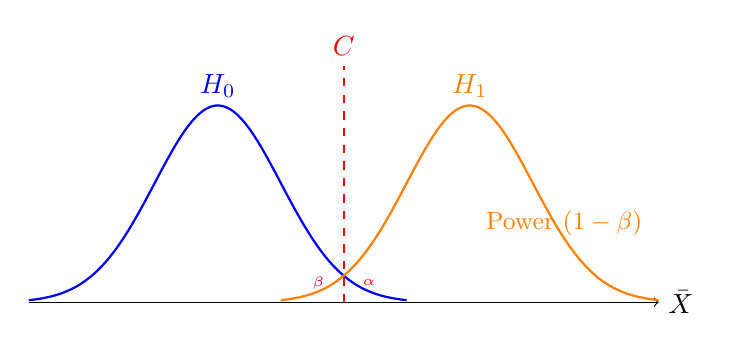
\begin{tikzpicture}[xscale=0.8, yscale=2.5] % פרופורציות גבוהות יותר
      % ציר X
      \draw[->] (-3,0) -- (7,0) node[right] {$\bar{X}$};
      
      % עקומה H0 (משמאל)
      \draw[thick, blue, domain=-3:3, samples=100] plot (\x, {exp(-(\x*\x)/2)});
      \node[blue] at (0,1.1) {$H_0$};
      
      % עקומה H1 (מימין)
      \draw[thick, orange, domain=1:7, samples=100] plot (\x, {exp(-(\x-4)^2/2)});
      \node[orange] at (4,1.1) {$H_1$};
      
      % קו קריטי C
      \draw[red, thick, dashed] (2,0) -- (2,1.2) node[above] {$C$};
      
      % שטחי טעות (צביעה וסימון)
      \node[red, font=\tiny] at (2.4,0.1) {$\alpha$};
      \node[purple, font=\tiny] at (1.6,0.1) {$\beta$};
      \node[orange, font=\small] at (5.5,0.4) {Power ($1-\beta$)};
    \end{tikzpicture}
    \end{english}
    \caption{התפלגות הדגימה תחת השערות חופפות ($H_0$ לעומת $H_1$).}
    \label{fig:power_graph}
\end{figure}

\subsection{שני מישורים בבדיקת השערות}

בכל בדיקת השערות קיימים שני מישורים נפרדים:

\begin{itemize}
\item \textbf{המצב במציאות}: האם השערת האפס $H_0$ נכונה או שגויה
\item \textbf{ההחלטה הסטטיסטית}: האם דוחים או לא דוחים את $H_0$
\end{itemize}

מאחר שהמצב האמיתי אינו ידוע לחוקרת,
ייתכנו טעויות בהחלטה.



\subsection{טעות מסוג ראשון \texorpdfstring{\textenglish{(Type I Error)}}{Type I Error}}
\subsubsection{הגדרה}
טעות מסוג ראשון מתרחשת כאשר דוחים את $H_0$ למרות שהיא נכונה.

\[
P(\text{טעות מסוג I}) = \alpha
\]

\subsubsection{פירוש אינטואיטיבי}
המדגם יצא קיצוני, אך בפועל אין אפקט אמיתי באוכלוסייה.

\subsubsection{מאפיינים חשובים}
\begin{itemize}
\item $\alpha$ נקבעת \textbf{מראש}
\item $\alpha$ אינה תלויה בתוצאת המדגם
\item $\alpha$ היא תכונה של המבחן
\end{itemize}



\subsection{\hebeng{טעות מסוג שני}{Type II Error}}

\subsubsection{הגדרה}
טעות מסוג שני מתרחשת כאשר לא דוחים את $H_0$ למרות ש-$H_1$ נכונה.

\[
P(\text{טעות מסוג II}) = \beta
\]

\subsubsection{פירוש אינטואיטיבי}
יש אפקט אמיתי באוכלוסייה,
אך המדגם לא היה קיצוני מספיק כדי לגלות אותו.

\subsubsection{מאפיינים חשובים}
\begin{itemize}
\item $\beta$ אינה נקבעת מראש
\item $\beta$ תלויה בתכנון המחקר
\item $\beta$ מתייחסת למצב שבו $H_1$ נכונה
\end{itemize}


\subsection{\hebeng{עוצמת המבחן}{Statistical Power}}

\subsubsection{הגדרה}
עוצמת המבחן היא ההסתברות לדחות את $H_0$
בהינתן ש-$H_1$ נכונה.

\[
\text{עוצמה} = 1 - \beta
\]

\subsubsection{פירוש אינטואיטיבי}
היכולת של המבחן \textbf{לגלות אפקט כאשר הוא באמת קיים}.

\subsubsection{דגש קריטי}
\begin{itemize}
\item עוצמה אינה תלויה במדגם הספציפי שיצא
\item עוצמה היא תכונה של \textbf{המבחן והתכנון}
\end{itemize}



\subsection{הגורמים המשפיעים על עוצמת המבחן}

\begin{itemize}
\item \textbf{גודל האפקט} – המרחק בין $H_0$ ל-$H_1$
\item \textbf{רמת המובהקות} $\alpha$
\item \textbf{גודל המדגם} $n$
\item \textbf{סטיית התקן באוכלוסייה}
\end{itemize}



\subsection{קשרים חשובים בין \texorpdfstring{$\alpha$}{alpha}, \texorpdfstring{$\beta$}{beta} ו-\texorpdfstring{$n$}{n}}

\begin{itemize}
\item הקטנת $\alpha$:
\begin{itemize}
\item מקטינה טעות מסוג ראשון
\item מגדילה טעות מסוג שני
\end{itemize}

\item הגדלת $n$:
\begin{itemize}
\item מקטינה טעות מסוג שני
\item מגדילה עוצמה
\item אינה משנה את $\alpha$
\end{itemize}

\item תמיד קיים \textbf{trade-off} בין $\alpha$ ל-$\beta$
\end{itemize}



\subsection{תכנון מחקר ועוצמה}

עוצמת המבחן ניתנת להשפעה \textbf{לפני איסוף הנתונים}.

\subsubsection{מה החוקרת יכולה לקבוע}
\begin{itemize}
\item גודל המדגם
\item רמת המובהקות $\alpha$
\item הגדרה תפעולית טובה של האפקט
\end{itemize}

\subsubsection{מה החוקרת אינה שולטת בו}
\begin{itemize}
\item האם $H_1$ נכונה במציאות
\item השונות האמיתית באוכלוסייה
\end{itemize}



\subsection{סוגי החלטות – סיכום לוגי}

\begin{english}
\begin{table}[H]
    \centering
    \renewcommand{\arraystretch}{2.0} % הגבהה של השורות למניעת המראה המעוך
    \setlength{\tabcolsep}{12pt}      % רווח בין העמודות
    \begin{tabular}{|c|c|c|}
    \hline
    \rowcolor[gray]{0.9} \textbf{Reality $\downarrow$ / Decision $\rightarrow$} & \textbf{Retain $H_0$} & \textbf{Reject $H_0$} \\ \hline
    \textbf{$H_0$ is True} & \cellcolor[HTML]{E2EFDA} Correct ($1-\alpha$) \checkmark & \cellcolor[HTML]{FCE4D6} Type I ($\alpha$) \ding{55} \\ \hline
    \textbf{$H_1$ is True} & \cellcolor[HTML]{FCE4D6} Type II ($\beta$) \ding{55} & \cellcolor[HTML]{E2EFDA} Power ($1-\beta$) \checkmark \\ \hline
    \end{tabular}
    \caption{Statistical Decision Matrix}
\end{table}
\end{english}

\subsection{ייצוג גרפי של הטעויות והעוצמה}
% שימוש ב-english כדי שה-TikZ והקיבוע [H] לא יתבלגנו
\begin{english}
\begin{figure}[H]
    \centering
    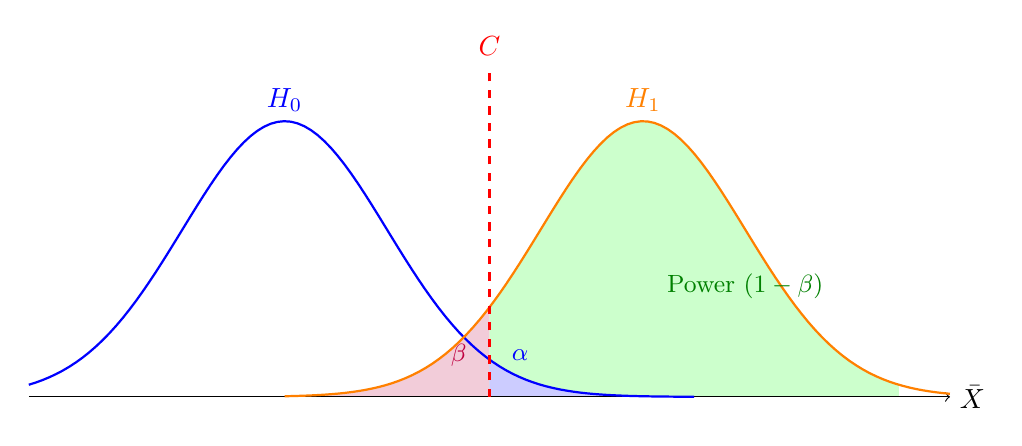
\begin{tikzpicture}[xscale=1.3, yscale=3.5, declare function={stdnorm(\x,\m)=exp(-0.5*((\x-\m)^2));}]
      
      % צביעת שטחים (Power, Beta, Alpha)
      \fill[green!20, domain=2:6, samples=100] plot (\x, {stdnorm(\x,3.5)}) -- (6,0) -- (2,0) -- cycle;
      \fill[purple!20, domain=0:2, samples=100] plot (\x, {stdnorm(\x,3.5)}) -- (2,0) -- (0,0) -- cycle;
      \fill[blue!20, domain=2:4, samples=100] plot (\x, {stdnorm(\x,0)}) -- (4,0) -- (2,0) -- cycle;

      % ציר X
      \draw[->] (-2.5,0) -- (6.5,0) node[right] {$\bar{X}$};
      
      % עקומה H0 (כחול)
      \draw[thick, blue, domain=-2.5:4, samples=100] plot (\x, {stdnorm(\x,0)});
      \node[blue, above] at (0,1) {$H_0$};
      
      % עקומה H1 (כתום)
      \draw[thick, orange, domain=0:6.5, samples=100] plot (\x, {stdnorm(\x,3.5)});
      \node[orange, above] at (3.5,1) {$H_1$};
      
      % קו קריטי C (אדום מקווקו)
      \draw[red, thick, dashed] (2,0) -- (2,1.2) node[above] {$C$};
      
      % סימוני אותיות בתוך השטחים - תיקון צבע לשחור-ירוק
      \node[blue, font=\small] at (2.3,0.15) {$\alpha$};
      \node[purple, font=\small] at (1.7,0.15) {$\beta$};
      \node[green!50!black, font=\small] at (4.5,0.4) {Power ($1-\beta$)};
      
    \end{tikzpicture}
    \caption{Visual representation of Type I/II errors and Statistical Power}
\end{figure}
\end{english}

\begin{figure}[H]
    \centering
    \includegraphics[width=0.9\textwidth]{figures/a_b_errors.png}
    \caption{Visual representation of Type I/II errors and Statistical Power}
\end{figure}

\subsection{דגש מסכם ליחידה}

\begin{itemize}
\item $\alpha$ מתארת טעות כאשר אין אפקט
\item $\beta$ מתארת פספוס של אפקט אמיתי
\item עוצמה היא היכולת לגלות אפקט
\item עוצמה אינה תוצאה – אלא תכנון
\end{itemize}

\subsection{חישובים מעשיים ביחידה 12}
כדי לחשב את גודל המדגם ($n$) הדרוש להשגת עוצמה מסוימת, נשתמש בנוסחה:
\[ n = \left( \frac{(Z_{1-\alpha} + Z_{1-\beta}) \cdot \sigma}{\mu_1 - \mu_0} \right)^2 \]
\textbf{דגש:} בבדיקה דו-צדדית, נשתמש ב-$Z_{1-\alpha/2}$ במקום ב-$Z_{1-\alpha}$.

\subsection*{שורת זהב ליחידה}

\begin{quote}
בדיקת השערות עוסקת בהחלטה,
אך יחידה 12 עוסקת באיכות ההחלטה.
\end{quote}


